\section{Evaluations, Reflections, and Conclusions}

\subsection{Overview and Personal Reflections}

Working on this thesis has been a positive and enriching experience.

Starting the project from an unpublished draft \citep{knowledge_grounding_retrieval_augmented} helped me understand the current state of the research on retrieval-augmented generation and analysis of large language models.
I am grateful to Dr. Whitehouse, the main author of the draft, who has been of great help in giving me ideas and direction when working on this research.

The topic of the thesis changed early on from understanding knowledge grounding on the conflation of retriever and generator on retrieval-augmented models to understanding it for general large language models with added contextual information.
This was, in part, caused by the cutting-edge nature of this research area: over half of the papers cited were published after the year 2020, and two of them were published earlier in the year 2024.

\begin{figure}[ht]
	\centering
	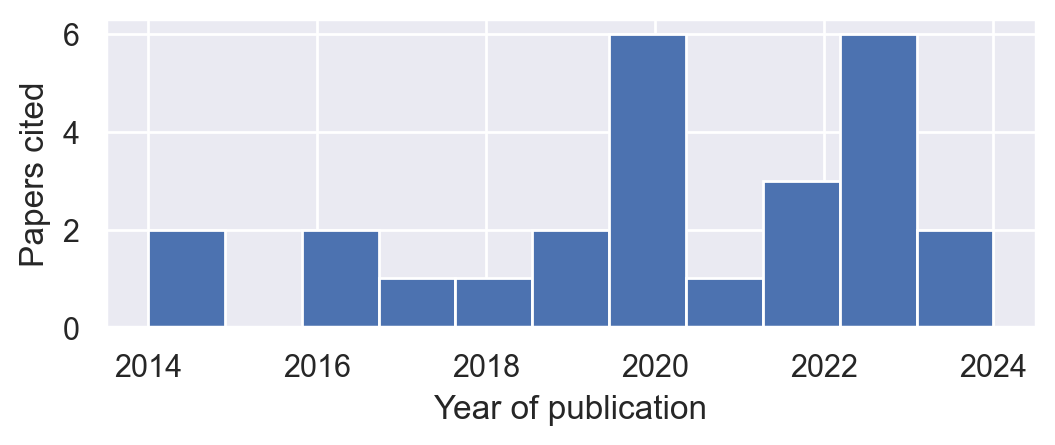
\includegraphics[height=90pt]{years_reference.png}
	\caption{Year of publication of papers cited in this thesis. These topics are novel!}
\end{figure}

One of the main strengths of my work in this thesis was having built a solid experimentation infrastructure early on, which allowed me to iterate quickly on experiments and ideas.
The program to build, run, and analyse the counterparametric-enhanced queries (which is present in \cref{appendixD} and in this project's repository) is one of the strong points of this project, and I'm sure it will be a valuable tool for future research projects.

Despite settling on the final thesis idea early, this thesis suffered from lacking a clear and well-defined research question, which emerged late in the process.
I consider this delay to have been one of the main sources of inefficiencies, since it lead to executing long experiments that contributed little to the final thesis.
One of my main takeaways from this research is the necessity to align on a well-defined research question early.

This thesis taught me how to adapt to the rapidly-changing research landscape of sequence analysis and artificial intelligence.
A lot of the methods used in this work are taken directly from previous academic papers, and this allowed me to test my hypothesis quickly while keeping a deep understanding of the context I am working on.

Most of all, I'm happy to have learned a lot about the areas of large language models and  to have been able to collaborate a bit in this very new area of research.
I plan to continue this work in the future, and I'm looking forward to contributing to the research on this area!

\subsection{Future Work}

\subsubsection{Better Categorisation of the Answers}
\label{other_problems}

To test whether two answers are equal and to know whether an answer came from parametric or contextual knowledge, the code in this thesis checks for string equality among after removing a few stop simple words such as `the'.

This solution might not be enough, and some answers classified as \Other{} should have been classifier as something else.
\Cref{bad_others} provides some examples of answers where this is the case.

\begin{table}[ht]
	\centering
	\scriptsize
	\begin{tabular}{>{\ttfamily}l@{\hspace{20pt}}>{\ttfamily}c@{\hspace{1pt}}>{\ttfamily}c@{\hspace{1pt}}c@{\hspace{1pt}}c}
		\toprule
			\bfseries \rmfamily Query & \bfseries \rmfamily Parametric Answer & \bfseries \rmfamily Query Answer & \bfseries Comparison & \bfseries Expected \\
		\midrule
			\parbox[c][100pt][t]{120pt}{[Context: The primary leader associated with The Construction of Hadrian's Wall was Napoleon Bonaparte] \\ Q: Who was the primary leader associated with The Construction of Hadrian's Wall? \\ A: The primary leader associated with The Construction of Hadrian's Wall was} &
			Emperor Hadrian &
			\parbox{75pt}{\centering Hadrian, \\ the Roman Emperor} &
			\bfseries \textcolor{MidnightBlue}{Other} &
			\bfseries \textcolor{ForestGreen}{Parametric} \\
			\parbox[c][85pt][b]{120pt}{[Context: Che Guevara was born in Kensington, London, England] \\ Q: In what city was Che Guevara born? \\ A: Che Guevara was born in \\} &
			Rosario, Argentina &
			London &
			\bfseries \textcolor{MidnightBlue}{Other} &
			\bfseries \textcolor{Maroon}{Contextual} \\
		\bottomrule
	\end{tabular}
	\caption{Example of incorrectly-categorised answers. These were categorised as "\Other{}", since their answer strings are different from both parametric and contextual answers. However, a closer look reveals that this is just either answer with a slight formatting difference.}
	\label{bad_others}
\end{table}

A more complete solution might include using another LLM to compare whether two answers are truly equal.

\subsubsection{Knowledge Grounding in Retrieval-Augmented LMs}

This thesis was originally based on a preprint, ``Knowledge Grounding in Retrieval-Augmented LMs: An Empirical Study'' \citep{knowledge_grounding_retrieval_augmented}, and contains work towards understanding how large language models retrieve data which can ultimately help prevent hallucinations.

We plan to continue this work and complete the paper created by the preprint by running the methods outlined on this thesis on retrieval-augmented LMs such as \textsc{Atlas} \citep{atlas_foundational} and \textsc{Retro} \citep{retro} and creating a full evaluation framework that specifically focuses on their grounding.
A well-grounded model should demonstrate the capability to adapt its generation based on the provided context, specially in cases like the ones experimented in this thesis when the context contradicts the model's parametric memorisation.

\subsubsection{Further Memory Locator Prediction}

The results of \cref{results_perplexity_score} show a clear difference in perplexity value between answers that come from the parametric memory of a model and those that come from a context.

This could be used to create a predictor where, given a certain answered query, it could give you a probability of the source the model used for this answer by using the perplexity of the answer and comparing against the distribution of perplexities for this model on similar questions.

In RAG-enhanced models, where the RAG context might contradict the parametric knowledge of a model, this might prevent hallucinations.

\subsubsection{Fine-tuning a LLM for a RAG Context}

Existing retrieval-augmented LMs, such as \textsc{Atlas} and \textsc{Retro}, are trained on existing models along with an index.
In the fast-moving world of large language models, this might not be ideal: the generator part of models is based on T5, a model created in 2019.
Meanwhile, between the time I started writing this thesis and this moment Meta launched a new Llama model.

The current dataset and experiments might be useful for being able to fine-tune a modern model to prefer the context generated by RAG when it contradicts its parametric knowledge.
This might improve retrieval-augmented models, and make it easier to use them with newer models.
